% !TEX root = catron-dissertation.tex
\epstopdfsetup{outdir=./images/05_synthetic_wavefront/}

\chapter{Synthetic Wavefront}
\label{chap:05_synthetic}

In the preceding chapter, the way that wavefront data appears in multidimensional spectra was shown using data acquired in Notre Dame’s White Field wind tunnel, for a representative wind-tunnel aero-optical test setup shown in Figure \ref{fig:02_typical_wavefront_system}.
The spectra and accompanying discussion showed how individual sources of optical aberration can be identified in the spectra, such as boundary-layer aero-optical signals, acoustic noise sources, mechanical vibration, etc.
In following chapters of this dissertation, filtering techniques will be presented for extracting or removing signals or noise sources from wavefront data such as shown in Chapter \ref{chap:03_optical_acoustics}.
As a first step towards this objective of developing and examining filtering approaches, this chapter presents methods used to construct a ``synthetic'' wavefront that contains typical optical and aero-optical signals, which will be used to test and examine different filtering techniques described in Chapter \ref{chap:06_single_filter}.

In order to best understand how some basic filters perform on a set of data, a fully known synthetic wavefront was generated such that all of the various components could be generated separately with the combined product filtered and compared to the synthetic wavefront containing only relevant aero-optical data.
This was done by constructing a multidimensional spectrum where each source component was separately generated with parameters that can be modified to alter the output signal as necessary.
The resulting multidimensional spectrum could then be used to create the equivalent spatial- and temporally-resolved wavefront signal in the physical domain by inverse Fourier transforming the spectrum.

This synthetic wavefront generation technique produces a qualitative representation that closely matches the measured wavefront but leaves room for improvement in producing a more physically accurate synthetic wavefront.
It should be stressed that, although physical models for the spectral behavior are presented for some of the signal components, the shape of the spectrum for each signal component was largely constructed to qualitatively match details observed in the spectra for experimental data such as shown in Chapter \ref{chap:03_optical_acoustics}.
This qualitative character to the constructed spectrum for some components should not influence the ability to use the synthesized spectral and wavefront data for examination of filtering approaches, since the constructed data still have the important behaviors exhibited by measured data.

The synthetic wavefront was generated to approximate the same sampling conditions used to acquire the data first presented in Section \ref{sect:03_summary}; these sampling conditions are reasonably typical for Shack-Hartmann wavefront measurements at the time of writing.
The sample rate was 200 m$^{-1}$ (i.e. 200 lenslets/m equivalent in the measurement beam) with 64 ($2^6$) samples in the spatial dimensions and 30,000 Hz with 8192 ($2^{13}$) samples in the temporal dimension.
% The speed of sound was chosen to be 340 m/s, with a Mach number of 0.6, and a boundary layer velocity of 163.2 m/s ($0.8U_\infty$).
Figure \ref{fig:05_dispersion_comp_real} shows the multidimensional spectra estimation of the measured wavefront that was used for the model.
\begin{figure}
  \centering
  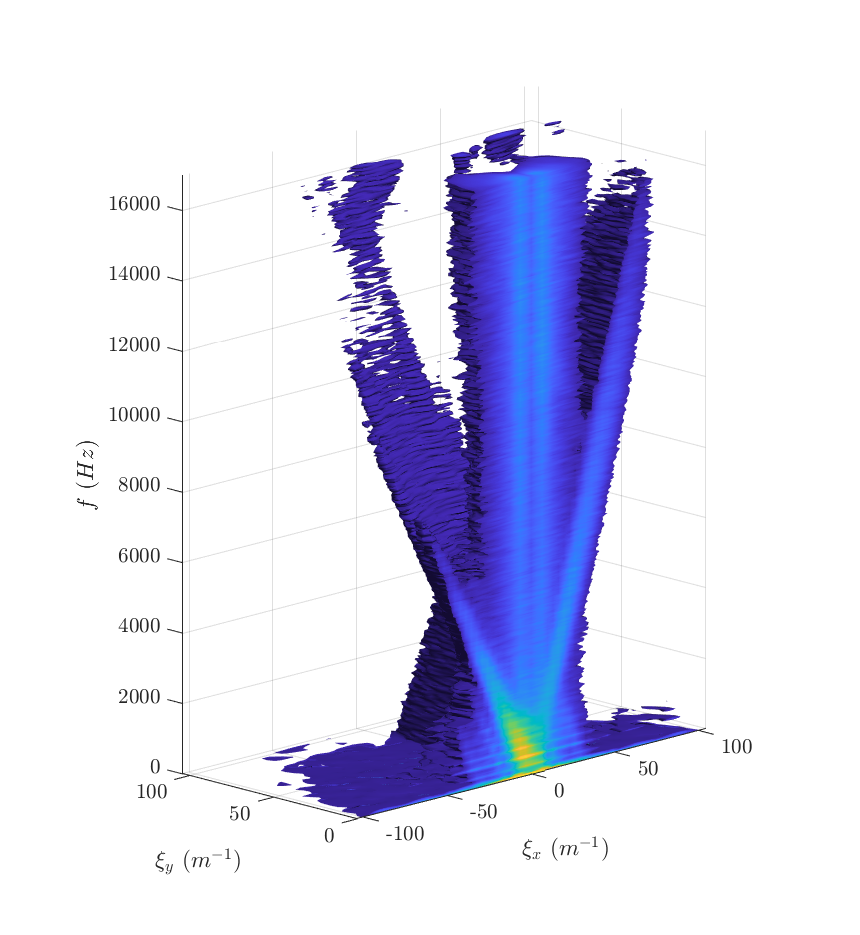
\includegraphics{../matlab/05_synthetic_wavefront/dispersion_comp_real.eps}
  \caption{Multidimensional spectral estimation that the synthetic wavefront is based on.}
  \label{fig:05_dispersion_comp_real}
\end{figure}
The optical wavefront was measured in the University of Notre Dame Whitefield wind tunnel at a Mach number of 0.6 with a 10-inch diameter beam.
The beam angle through the test section was $90^\circ$.

The signals that were assumed to be statistically independent from one another, such as the boundary layer signal, were converted into dimensional space separately and then summed together, while signals that were assumed to be related to one another, such as the sound and vibration components, were first summed together in frequency space.
Figure \ref{fig:05_synthetic_dispersion_input} shows the input dispersion plot with each signal component separately colored.
\begin{figure}
 \centering
 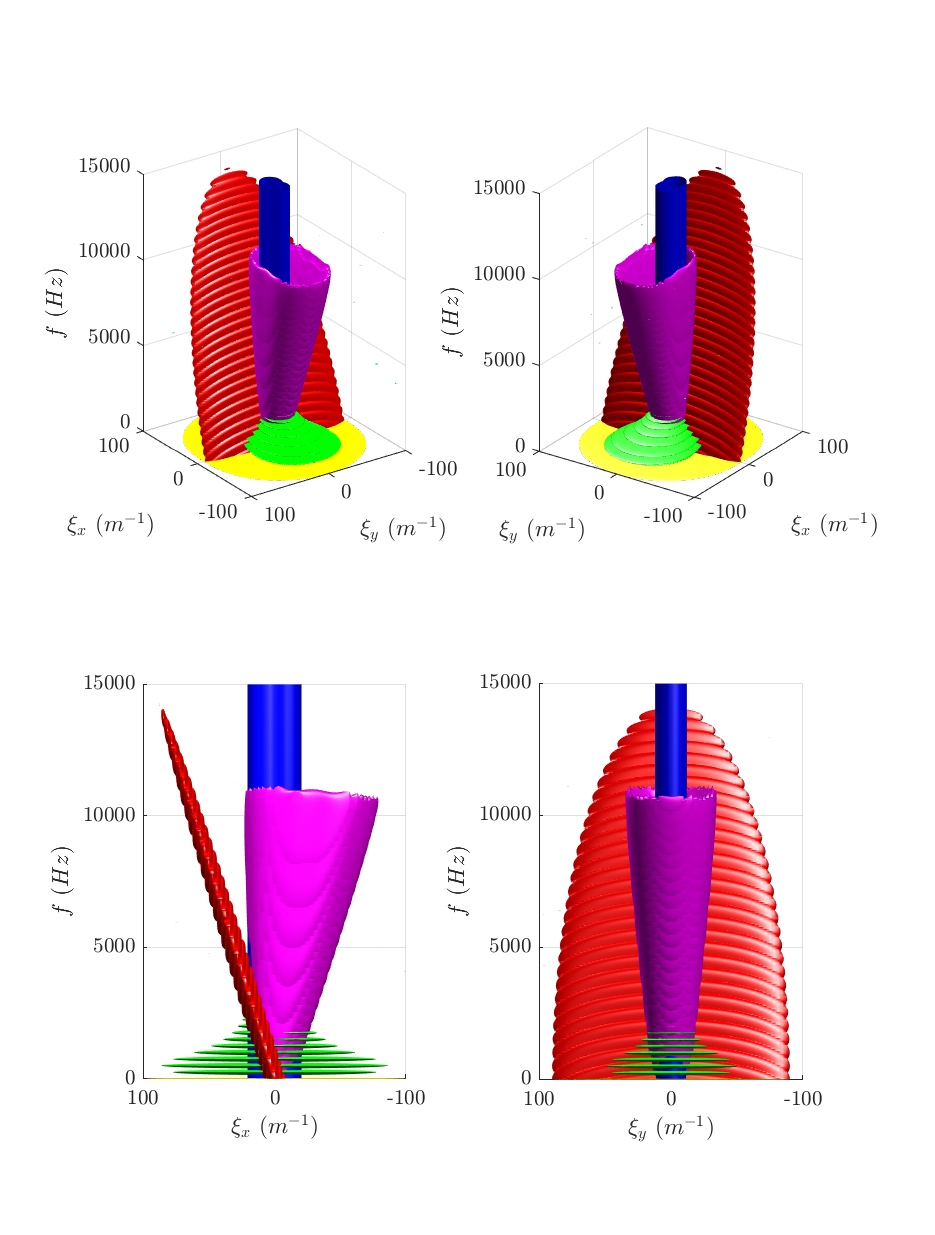
\includegraphics{../matlab/05_synthetic_wavefront/synthetic_wavefront.eps}
 \caption{Synthetic wavefront input dispersion plot of an aero-optical signal and various signal corruption components.  The aero-optical signal is shown in red, the stationary modes in blue, duct acoustics in magenta, blade-passing frequency related corruption in green, slowly varying mean-lensing in yellow, and background in cyan.}
 \label{fig:05_synthetic_dispersion_input}
\end{figure}
The aero-optical signal is shown in red, the stationary modes in blue, duct acoustics in magenta, blade-passing frequency related noise in green, slowly varying mean-lensing in yellow, and background noise in cyan.

\section{General Spectrum Construction}
The general process of developing most of the component signals was to determine an approximate shape, normalize it in the appropriate dimensions, and scale the result by using a function derived from a hyperbola,
\begin{equation}
 \frac{\log_{10}(WF)-b}{b^2}-\frac{\xi_{\rho_N}^2}{a^2} = 1 \textrm{,}
 \label{eqn:05_scaling_hyperbola}
\end{equation}
such that the signal strength at unity of the normalized radial frequency, $\log_{10}(WF(\xi_{\rho_N}=1))$, and the limiting slope, $a/b$, are inputs.
This results in the signal strength of the wavefront being
\begin{equation}
 \log_{10}(WF) = b-\sqrt{\frac{\xi_{\rho_N}^2}{m^2}+b^2} \textrm{,}
 \label{eqn:05_wavefront_strength}
\end{equation}
where
\begin{equation}
 b = \frac{1}{2\log_{10}(WF(\xi_{\rho_N}=1))}\cdot\left(\log_{10}(WF(\xi_{\rho_N}=1))^2-\frac{1}{m^2}\right) \textrm{.}
 \label{eqn:05_wavefront_strength_b}
\end{equation}
% The code used to generate the synthetic wavefront used in this section is shown in Appendix \ref{code:sc_synthetic_wavefront}.

\section{Aero-Optical Signal}
The aero-optical signal was generated to approximate an optical beam passing perpendicularly through a test section with boundary layers on each of the test section walls.
An ellipsoid was chosen to approximate the boundary-layer signal because it is the simplest shape that best resembles the aero-optical signal in Figure \ref{fig:05_dispersion_comp_real}.
This signal was approximated by creating an ellipsoid,
\begin{equation}
  \xi_{\rho_N}^2 = (\xi_{x,R}/a_x)^2+(\xi_{y,R}/a_y)^2+(f_R/a_t)^2
\end{equation}
which had been rotated into the plane representing the boundary-layer's dispersion velocity,
\begin{equation}
  \left[\begin{array}{c} \xi_{x,R} \\ \xi_{y,R} \\ f_R \end{array}\right] = \left[\begin{array}{c c c} \cos\theta_u & 0 & \sin\theta_u \\ 0 & 1 & 0 \\ -\sin\theta_u & 0 & \cos\theta_u \end{array}\right]\left[\begin{array}{c} \xi_{x} \\ \xi_{y} \\ f \end{array}\right]
\end{equation}
where $\theta_u=\tan^{-1}(-1/u_{BL})$.
Equations \ref{eqn:05_wavefront_strength} and \ref{eqn:05_wavefront_strength_b} were then used to calculate the multidimensional spectrum of the boundary layer signal.
% The code used to generate the multidimensional spectrum of the boundary layer signal are shown in lines 18-31 of Appendix \ref{code:sc_synthetic_wavefront} and
The values used are shown in Table \ref{tab:05_boundary_layer}.
In Figure \ref{fig:05_synthetic_dispersion_input} the aero-optical signal is shown in red.
\begin{table}
  \centering
  \caption{Values used in the construction of the multidimensional spectrum for the boundary layer signal}
  \begin{tabular}{c c}
    Variable & Value \\
    \hline \hline
    $a_x$ & 8 \\
    $a_y$ & 90 \\
    $a_t$ & 175 \\
    $m$ & -0.13 \\
    $u_{BL}$ & 163.2 m/s \\
    $\log_{10}(WF(\xi_{\rho_N}=1))$ & -14.5
  \end{tabular}
  \label{tab:05_boundary_layer}
\end{table}

\section{Stationary Mode Signals}
The collection of stationary modes is a temporally constant signal at low spatial frequencies that is often has a cross-section in the plane of spatial-frequencies that is circular.
In the particular case that is being modeled, the stationary modes have a cross-section of two circular regions offset along the $\xi_x$-axis that just overlap one another.
A smooth function was chosen to approximate this overlapping circle type stationary mode,
\begin{equation}
 \xi_{\rho_N} = \frac{\xi_\rho}{\xi_{\rho_0}\sqrt{10-6\cos{(2\xi_\theta+\pi)}}} \textrm{.}
 \label{eqn:05_epicycloid_simple}
\end{equation}
This spectrum for the stationary modes component is shown in blue in Figure \ref{fig:05_synthetic_dispersion_input}.
 % and the relevant code shown in Lines 33-40 of Appendix \ref{code:sc_synthetic_wavefront}.
Table \ref{tab:05_stationary_modes} shows the values used in generating the spectrum.
\begin{table}
  \centering
  \caption{Values used in the construction of the multidimensional spectrum for the signal of the stationary modes}
  \begin{tabular}{c c}
    Variable & Value \\
    \hline \hline
    $m$ & -0.175 \\
    $\xi_{\rho_0}$ & 5 \\
    $\log_{10}(WF(\xi_{\rho_N}=1))$ & -14.5
  \end{tabular}
  \label{tab:05_stationary_modes}
\end{table}

\section{Sound and Vibration Signals}
The sound and vibrating component signals are comprised of two parts.
The first of these is the blade-passing frequency and its harmonic disturbances (shown in green in Figure \ref{fig:05_synthetic_dispersion_input}) and the second is the acoustic duct modes (shown in magenta).

\subsection{Blade-Passing Frequency Disturbance}
Like the stationary modes, the blade-passing frequency disturbances were modeled with the same cross-sectional shape as the stationary mode, Equation \ref{eqn:05_epicycloid_simple}, but as narrow-band discs,
\begin{equation}
  \xi_{\rho_N}^2 = \frac{\sqrt{\xi_x^2+(AR\xi_y)^2}}{\xi_{\rho,BPF}\sqrt{10-6\cos(2\xi_\theta+\pi)}}+\left(\frac{f\pm BPF n}{f_T}\right)^2
  \label{eqn:05_blade_passing_frequency}
\end{equation}
where $AR$ is the aspect ratio of the cross-sectional shape, $n$ is the harmonic number, $f_T$ is the disc thickness, and $\xi_{rho,BPF}$ is
\begin{equation}
  \xi_{rho,BPF} = \frac{\xi_{\rho_0}}{\sqrt{1+\frac{BPF n-BPF}{f_c}}}
\end{equation}
where $f_c$ is the effectively cutoff frequency for modulating the strength of each disc as the harmonic number increased from $n=0.5$ to $n=5$ in steps of 0.5.
% The code for the blade-passing frequency disturbances is shown in Lines 42-60 of Appendix \ref{code:sc_synthetic_wavefront} with
A list of values is shown in Table \ref{tab:05_bpf}.
\begin{table}
  \centering
  \caption{Values used in the construction of the multidimensional spectrum for the blade-passing frequency disturbance}
  \begin{tabular}{c c}
    Variable & Value \\
    \hline \hline
    $AR$ & 1 \\
    $BPF$ & 500 Hz \\
    $f_c$ & 500 Hz \\
    $f_T$ & 100 Hz \\
    $m$ & -0.13 \\
    $\xi_{\rho_0}$ & 20 \\
    $\log_{10}(WF(\xi_{\rho_N}=1))$ & -14
  \end{tabular}
  \label{tab:05_bpf}
\end{table}


\subsection{Acoustic Cone}
The acoustic duct mode disturbances form a cone which in the $f-\xi_x$ plane is defined by the lines $u\pm c$, while in the $f-\xi_y$ plane is defined by the speed of sound.
At each temporal frequency step an ellipse was defined based on the constraining lines and the distance to that ellipse used to calculate a normalized radial frequency,
\begin{equation}
  \xi_{\rho_N}^2 = \frac{\sqrt{(\xi_x-\xi_{x_0})^2+(\xi_y-\xi_{y_0})^2}}{\sqrt{\xi^2_{x_a}\cos^2\xi_\theta+\xi^2_{y_a}\sin^2\xi_\theta-1}} \frac{\sqrt{\xi^2_{x_a}\cos^2\xi_\theta+\xi^2_{y_a}\sin^2\xi_\theta}}{\xi_{\rho_T}} \textrm{,}
\end{equation}
where $\xi_{x_0}$ and $\xi_{y_0}$ are the midpoint between the sonic lines in the x and y directions as a function of $f$, $\xi_{x_a}$ and $\xi_{y_a}$ are the distances from the midpoint to the sonic lines as a function of $f$, and $\xi_{\rho_T}$ is the thickness of the ellipse.
The strength of the disturbance was decreased logarithmically as a function of $|f|$ from $f=0$ to $f=f_s/2$ with Equation \ref{eqn:05_wavefront_strength_b} becoming,
\begin{equation}
  b(f) = \frac{1}{2b_0(f)}\left(b_0^2(f)-\frac{1}{m^2}\right) \textrm{,}
\end{equation}
where
\begin{equation}
  \begin{aligned}
    b_0(f) =& \frac{\log_{10}(WF(\xi_{\rho_N}=1,f=f_s/2))-\log_{10}(WF(\xi_{\rho_N}=1,f=0))}{f_s/2}|f| \\ &+\log_{10}(WF(\xi_{\rho_N}=1,f=f_0)) \textrm{.}
  \end{aligned}
\end{equation}

Two low-pass spatial filters (more discussion in Chapter \ref{chap:06_single_filter}) were used to replicate some of the signal attenuation that happens at the low spatial frequencies in the x-direction.
First a low-pass filter in $\rho$ was used,
\begin{equation}
  WF = WF\sqrt{\frac{1}{1+\left(\frac{\xi_\rho}{\xi_{c_\rho}}\right)^2}} \textrm{,}
\end{equation}
followed by a low-pass filter in the x-direction,
\begin{equation}
  WF = WF\sqrt{\frac{1}{1+\left(\frac{\xi_x}{\xi_{c_x}}\right)^2}} \textrm{.}
\end{equation}
The values used in creating the spectrum are shown in Table \ref{tab:05_cone}.
 % and the code is shown in lines 74-93 of Appendix \ref{code:sc_synthetic_wavefront}.
\begin{table}
  \centering
  \caption{Values used in the construction of the multidimensional spectrum for the acoustic cone disturbance}
  \begin{tabular}{c c}
    Variable & Value \\
    \hline \hline
    $m$ & -0.3 \\
    $\xi_{c_x}$ & 115 m$^{-1}$ \\
    $\xi_{c_\rho}$ & 200 m$^{-1}$ \\
    $\xi_{\rho_T}$ & 8 m$^{-1}$ \\
    $\log_{10}(WF(\xi_{\rho_N}=1,f=0))$ & -13 \\
    $\log_{10}(WF(\xi_{\rho_N}=1,f=f_s/2))$ & -16
  \end{tabular}
  \label{tab:05_cone}
\end{table}

\section{Mean-Lensing Signal}
The mean lensing part of the optical signal is the integrated effect of steady optical aberrations added by lenses, mirror, windows, etc, in the beam path.
The aberrations are effectively random and a physical model cannot be developed for them.
The mean-lensing signal (shown in yellow in Figure \ref{fig:05_synthetic_dispersion_input}) uses same cross-sectional as the blade-passing frequency disturbances and represents the slowly varying spatial disturbance,
\begin{equation}
  \xi_{\rho_N}^2 = \frac{\sqrt{\xi_x^2+(AR\xi_y)^2}}{\xi_{\rho_0}\sqrt{10-6\cos(2\xi_\theta+\pi)}}+\left(\frac{f}{f_T}\right)^2 \textrm{.}
  \label{eqn:05_mean_lensing}
\end{equation}
% The relevant code is shown on lines 62-72 of Appendix \ref{code:sc_synthetic_wavefront} with values shown in Table \ref{tab:05_mean_lensing}.
Table \ref{tab:05_mean_lensing} shows a list of the values used in creating this component of the wavefront signal.
\begin{table}
  \centering
  \caption{Values used in the construction of the multidimensional spectrum for the mean-lensing disturbance}
  \begin{tabular}{c c}
    Variable & Value \\
    \hline \hline
    $AR$ & 0.55 \\
    $f_T$ & 50 Hz \\
    $m$ & -0.5 \\
    $\xi_{\rho_0}$ & 25 \\
    $\log_{10}(WF(\xi_{\rho_N}=1))$ & -14.5
  \end{tabular}
  \label{tab:05_mean_lensing}
\end{table}

\section{Background Noise Signal}
Background noise in the wavefront data originates from sources which are random in nature.
The background noise disturbance (with a few small spots shown in cyan in Figure \ref{fig:05_synthetic_dispersion_input}) was simulated using normally distributed random noise with a mean noise level, $\mu(\log_{10}(WF))=-18$, and deviation, $\sigma(\log_{10}(WF))=0.75$.
% The relevant code is shown in lines 95-100 of Appendix \ref{code:sc_synthetic_wavefront}.

\section{Synthetic Wavefront Creation}
A synthetic signal can be created from a auto-spectral density by solving for $x$ in Equation \ref{eqn:04_basic_sxx} and using the Inverse Fourier Transform,
\begin{equation}
 x(t) = \real\left[\ifft\left\{\sqrt{S_{xx}\cdot N\cdot f_{samp}}\cdot\exp{i\phi}\right\}\right] \textrm{,}
 \label{eqn:05_ifft}
\end{equation}
where $\real$ is the real component and $\phi$ is a random set of phases for each point in the measurement space.
As shown previously this relation can be extended into $n$-dimensions,
\begin{equation}
 f(\mathbf{x}) = \real\left[\ifftn\left\{\sqrt{\mathbf{S_{xx}}\cdot\prod{\overrightarrow{N}\cdot \overrightarrow{f}_{samp}}}\cdot\exp{i\mathbf{\phi}}\right\}\right] \textrm{.}
 \label{eqn:05_ifftn}
\end{equation}
Care should be taken when constructing the random set of phases, as the zero-frequency component has zero phase, $\phi(0,0,0) = 0$, and the phases on either side of it are conjugates of one another, $\phi(\pm\xi_x,\pm\xi_y,\pm f)=-\phi(\mp\xi_x,\mp\xi_y,\mp f)$.
% The code for creating a wavefront from a multidimensional spectrum is shown in lines 196-202 of Appendix \ref{code:sc_synthetic_wavefront} and is specifically creating the wavefront for the aero-optical signal but other signals are generated using the same basic code.
% Note that the first three lines are to get the set of phases properly configured that creates conjugate phases rotated about the origin.

It was assumed that the aero-optical signal, the stationary modes, the background noise, and the sound and vibration combination of modes were statistically independent of one another and, as such, could be separately transformed into physical space.
The components of the sound and vibration sources, the blade-passing frequency, the acoustic cone, and the mean-lensing, were assumed to be related to one another and thus were summed together in frequency space prior to being transformed into physical space.
Once the separate components were in physical space the total wavefront was obtained by summing up the separate components with the aero-optical signal saved along side the total wavefront.
Some frames from the synthetic wavefront are shown in Figure \ref{fig:05_synthetic_frames} with the total wavefront shown on top and the aero-optical only signal shown on the bottom.
\begin{figure}
 \centering
 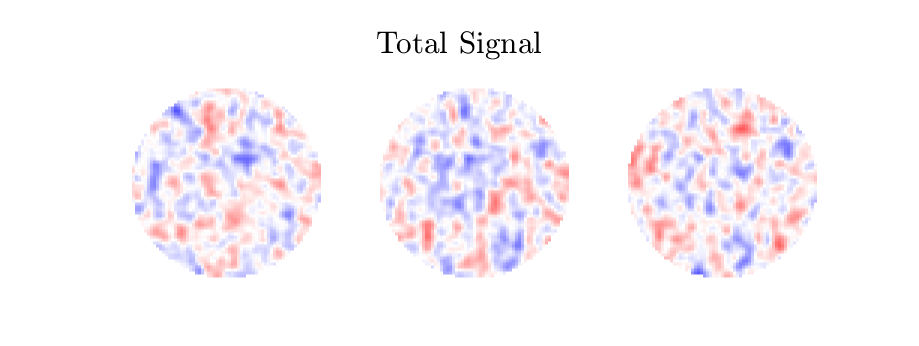
\includegraphics{../matlab/05_synthetic_wavefront/synthetic_frames_total.eps}
 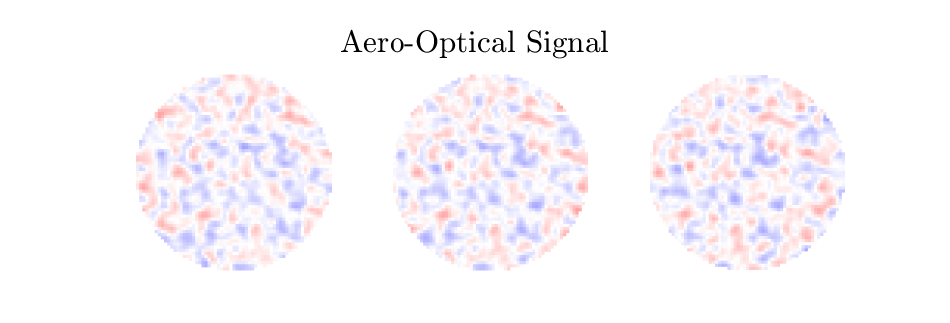
\includegraphics{../matlab/05_synthetic_wavefront/synthetic_frames_ao.eps}
 \caption{Sample frames from the synthetic wavefront with the total wavefront signal on top and the aero-optical only signal bottom.  Flow is from right to left.}
 \label{fig:05_synthetic_frames}
\end{figure}
Flow is from right to left.
The aero-optical signal is noticeable to some degree in the total wavefront signal, but can be overpowered by the various noise sources.

\section{Comparison to Measured Data}
A multidimensional spectral plot of the total synthetic wavefront is shown in Figure \ref{fig:dispersion_comp_synthetic}.
\begin{figure}
 \centering
 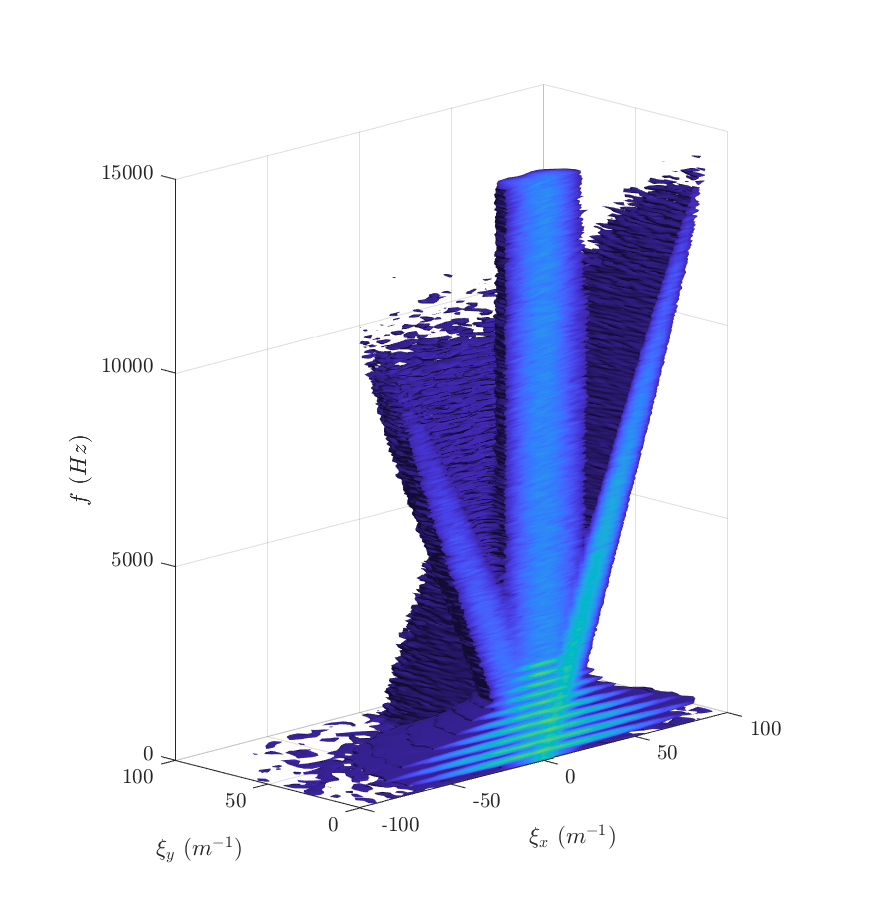
\includegraphics{../matlab/05_synthetic_wavefront/dispersion_comp_synthetic.eps}
 \caption{Synthetic wavefront output dispersion plot of an aero-optical signal and various signal corruption components.}
 \label{fig:dispersion_comp_synthetic}
\end{figure}
In this view the aero-optical signal is more noticeable but there still remains some significant overlap with the various noise sources.
While the mean-lensing component is not as visible in this isosurface, the rest of the dispersion plot in a good representation of the input dispersion plot shown in Figure \ref{fig:05_synthetic_dispersion_input}.
The blade-passing frequency was depicted as symmetric in the synthetic wavefront while measured data (shown in Figure \ref{fig:04_dispersion_3d}) shows more signal on the side traveling in the direction of flow.
The harmonics of the BPF are more on the upstream traveling side of the dispersion and are a little less pronounced in the measured data.
The total synthetic wavefront has a $\opdrms$ of $0.0112\pm0.0006\mu m$ with the aero-optical only signal having a $\opdrms$ of $0.0073\pm0.0003\mu m$.
The measured wavefront presented in Figure \ref{fig:04_dispersion_3d} had a $\opdrms$ of $0.0874\pm0.0263\mu m$.
The overall $\opdrms$ of the synthetic wavefront was $12.8\%$ when compared to the measured wavefront indicating that the algorithms used to generate the wavefront are not representative of reality and can provide a future path of research in order to produce more realistic synthetic wavefronts.
